\documentclass[a4paper,12pt]{article}
\usepackage[T2A]{fontenc}
\usepackage[utf8]{inputenc}
\usepackage[russian]{babel}
\usepackage{graphicx}
\usepackage{float}
\usepackage{amsmath}
\usepackage[margin=2.5cm]{geometry}
\graphicspath{{./}}
\begin{document}
\section*{Приложение. Графики и результаты}

\begin{figure}[H]\centering
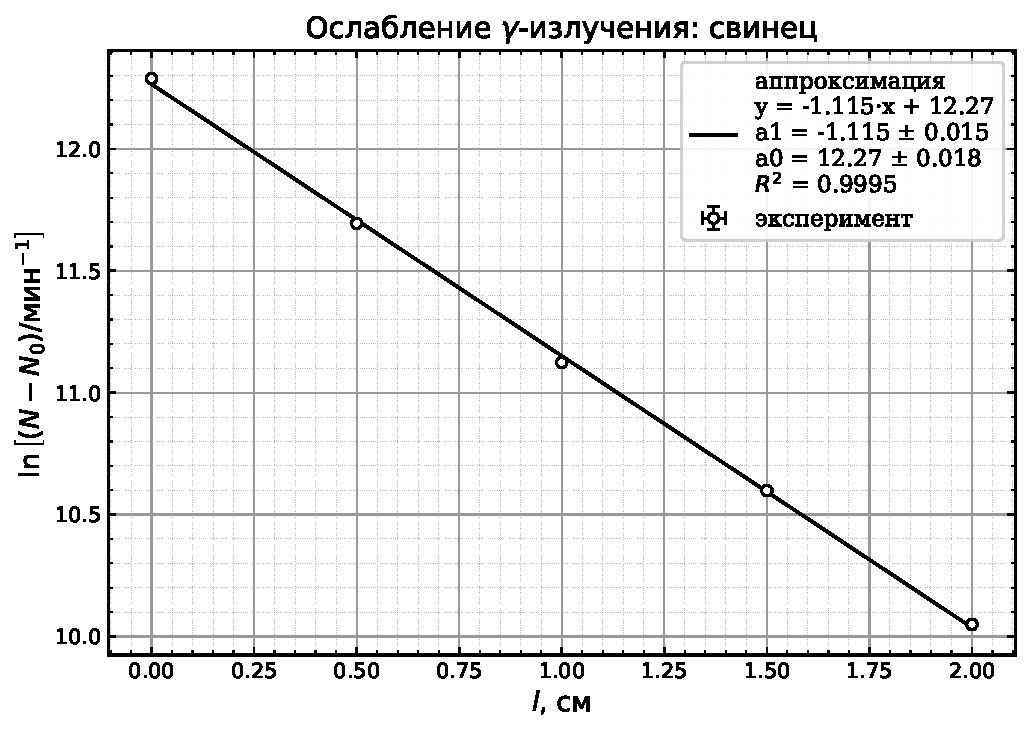
\includegraphics[width=0.82\textwidth]{fig_5_1_pb.pdf}
\caption{Ослабление $\gamma$-излучения $^{137}$Cs в свинце, $\rho=11{,}34$~г/см$^3$.}
\end{figure}
\begin{center}\small
$\mu=1.115\pm0.061$~см$^{-1}$;\quad $\mu/\rho=0.0983\pm0.0054$~см$^2$/г (табл. 0.1107, откл. $-11.2\%$);\quad $d_{1/2}=6.22\pm0.34$~мм;\quad $R^2=0.9995$.
\end{center}

\begin{figure}[H]\centering
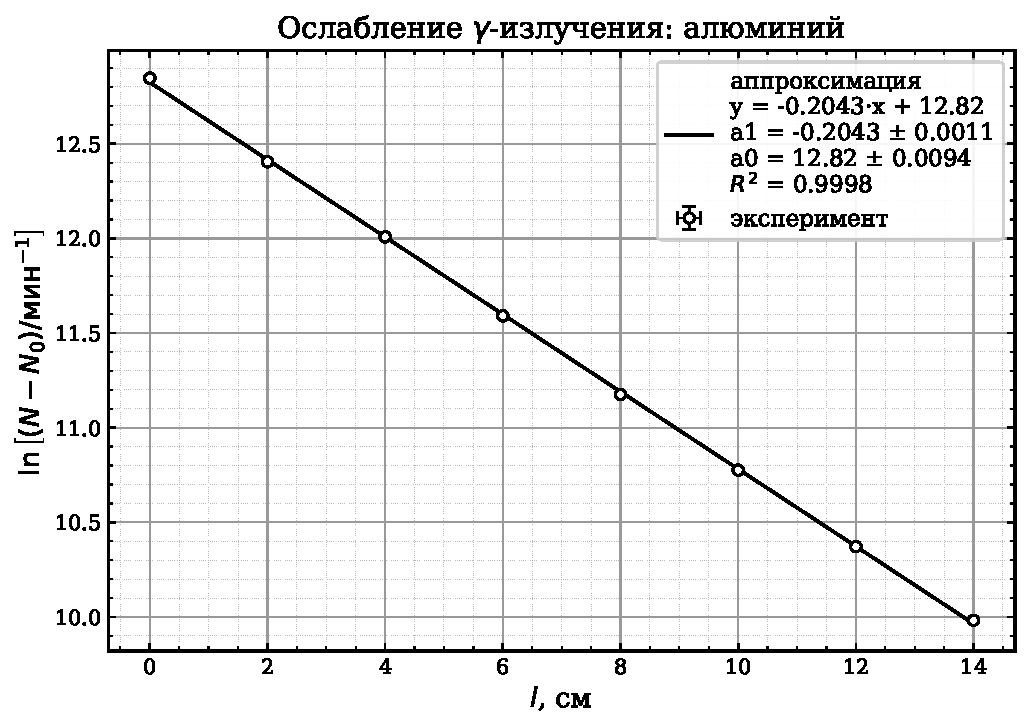
\includegraphics[width=0.82\textwidth]{fig_5_1_al.pdf}
\caption{Ослабление $\gamma$-излучения $^{137}$Cs в алюминии, $\rho=2{,}70$~г/см$^3$.}
\end{figure}
\begin{center}\small
$\mu=0.204\pm0.009$~см$^{-1}$;\quad $\mu/\rho=0.0757\pm0.0033$~см$^2$/г (табл. 0.0743, откл. $+1.8\%$);\quad $d_{1/2}=33.93\pm1.47$~мм;\quad $R^2=0.9998$.
\end{center}

\begin{figure}[H]\centering
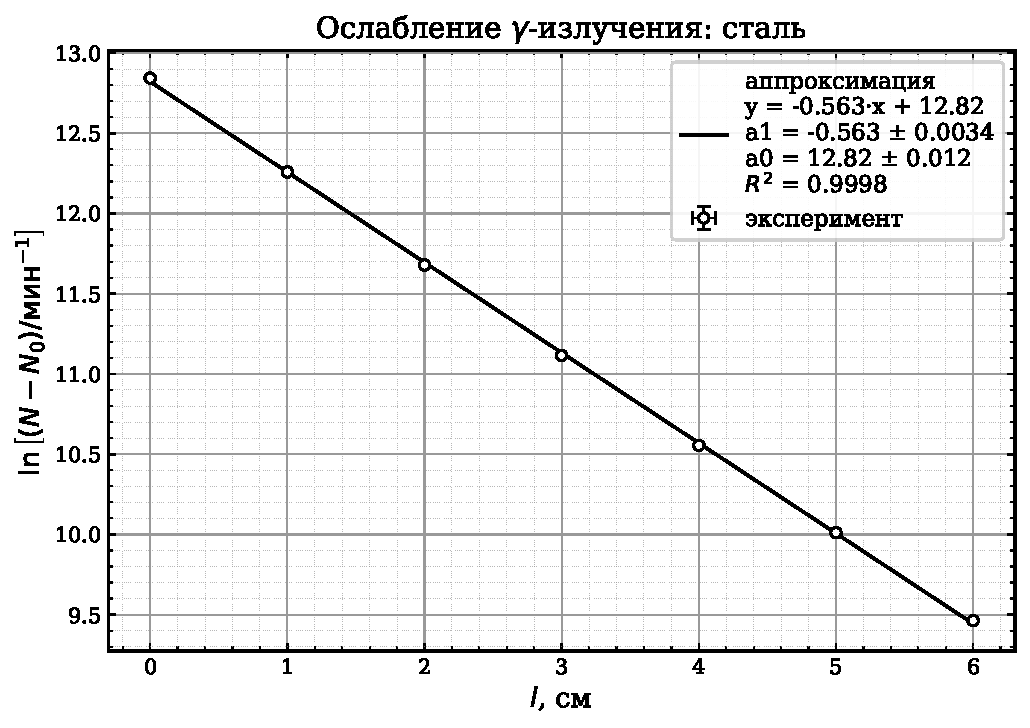
\includegraphics[width=0.82\textwidth]{fig_5_1_fe.pdf}
\caption{Ослабление $\gamma$-излучения $^{137}$Cs в стали, $\rho=7{,}87$~г/см$^3$.
Точка $l=7$~см исключена как промах: скорость счёта растёт с толщиной.}
\end{figure}
\begin{center}\small
$\mu=0.563\pm0.018$~см$^{-1}$;\quad $\mu/\rho=0.0715\pm0.0023$~см$^2$/г (табл. 0.0731, откл. $-2.1\%$);\quad $d_{1/2}=12.31\pm0.40$~мм;\quad $R^2=0.9998$.
\end{center}

\begin{figure}[H]\centering
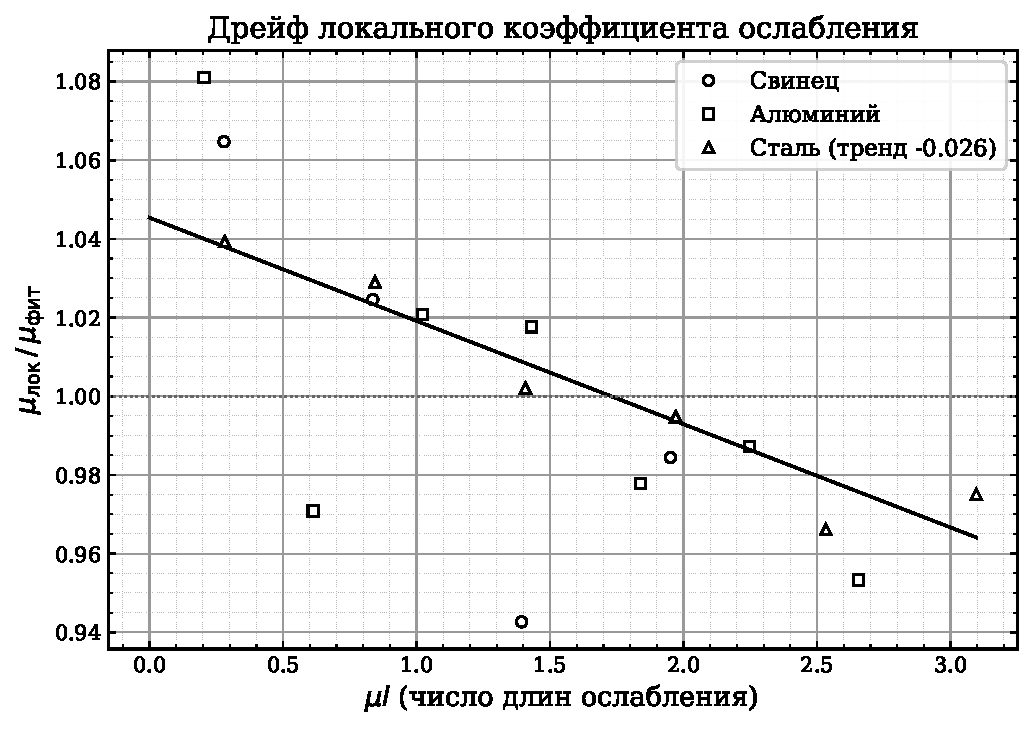
\includegraphics[width=0.82\textwidth]{fig_5_1_buildup.pdf}
\caption{Дрейф локального коэффициента ослабления --- накопление рассеянного
излучения. Для чистой экспоненты ожидалась бы горизонталь $\mu_\text{лок}/\mu_\text{фит}=1$.
Трендовая прямая проведена только для стали, где падение монотонно; для свинца
и алюминия показаны только точки.}
\end{figure}


\begin{center}\small
\textbf{Определение средней энергии источника.}
Обратная интерполяция измеренных $d_{1/2}$ по табличной зависимости $d_{1/2}(E)$:\\[2pt]
$E_{\mathrm{Pb}}=0.732\pm0.034$;\quad $E_{\mathrm{Fe}}=0.692\pm0.047$;\quad $E_{\mathrm{Al}}=0.637\pm0.061$~МэВ.\\[2pt]
Среднее: $\boxed{E=0.69\pm0.03~\text{МэВ}}$;\quad
табличное для $^{137}$Cs --- $0{,}662$~МэВ, отклонение
$+3.8\%$ ($0.9\sigma$).
\end{center}

\begin{center}\small
Погрешность $\mu$ --- полный бюджет: разброс точек
0.5--1.3\%,
толщина ($\delta d=0{,}005$~см) 0.2--1.0\%,
плотность 0.2--1.3\%,
билдап 2.9--5.2\%.
Табличные $d_{1/2}$ --- de.wikipedia.org/wiki/Halbwertsschicht,
интерполяция на $E_\gamma=662$~кэВ между узлами $0{,}6$ и $0{,}8$~МэВ.
\end{center}

\end{document}
